\documentclass[11pt]{article}
\usepackage[a4paper, margin=2cm]{geometry}
\usepackage[utf8]{inputenc}
\usepackage{babel}
\usepackage[spanish]{layout}
\usepackage[article]{ragged2e}
\usepackage{textcomp}
\usepackage{amsmath}
\usepackage{amssymb}
\usepackage{amsfonts}
\usepackage{proof}
\usepackage{enumerate}
\usepackage{graphicx}
\usepackage{multirow}
\usepackage{caption}
\usepackage{subcaption}

\setlength{\parindent}{0pt}

\title{
    Entrega 7 \\
    \large Sistemas Operativos II}
\author{Mellino, Natalia \and Farizano, Juan Ignacio}

\date{}

\begin{document}
\maketitle

\noindent\rule{\textwidth}{1pt}

\section*{Ejercicio 1}

Para un proceso externo el segmento de texto de un programa es de sólo lectura,
por lo tanto si un proceso intenta escribir en él se producirá una excepción de
\textbf{violación de seguridad}, llevando típicamente a la terminación del proceso.

\section*{Ejercicio 2}

Las entradas de la tabla de paginación están definidas en el archivo
\texttt{machine/translation\_entry.hh}, ahí podemos cómo está conformada, 
escribimos el contenido de las entradas pedidas en la siguiente tabla.

\begin{table}[h!]
  \begin{center}
        \begin{tabular}{|c|c|c|c|c|c|c|}
            \hline
            Proceso & virtualPage & physicalPage & valid & readOnly & use  & dirty \\ \hline
            A       & 10          & 5            & false & true     & true & false \\ \hline
            B       & 15          & 5            & false & true     & true & false \\ \hline
        \end{tabular}
  \end{center}
\end{table}

\section*{Ejercicio 3}

Si no se utilizara CoW, al momento que uno de los procesos escriba en una de
las páginas, se estaría modificando el contenido para ambos, ya que al 
hacer \emph{fork} ambos procesos comparten la/s misma/s página/s de memoria. Esto
podría causar comportamiento erróneo en la ejecución del otro proceso.

\newpage
\section*{Ejercicio 4}

\begin{figure}[h!]
  \begin{center}
    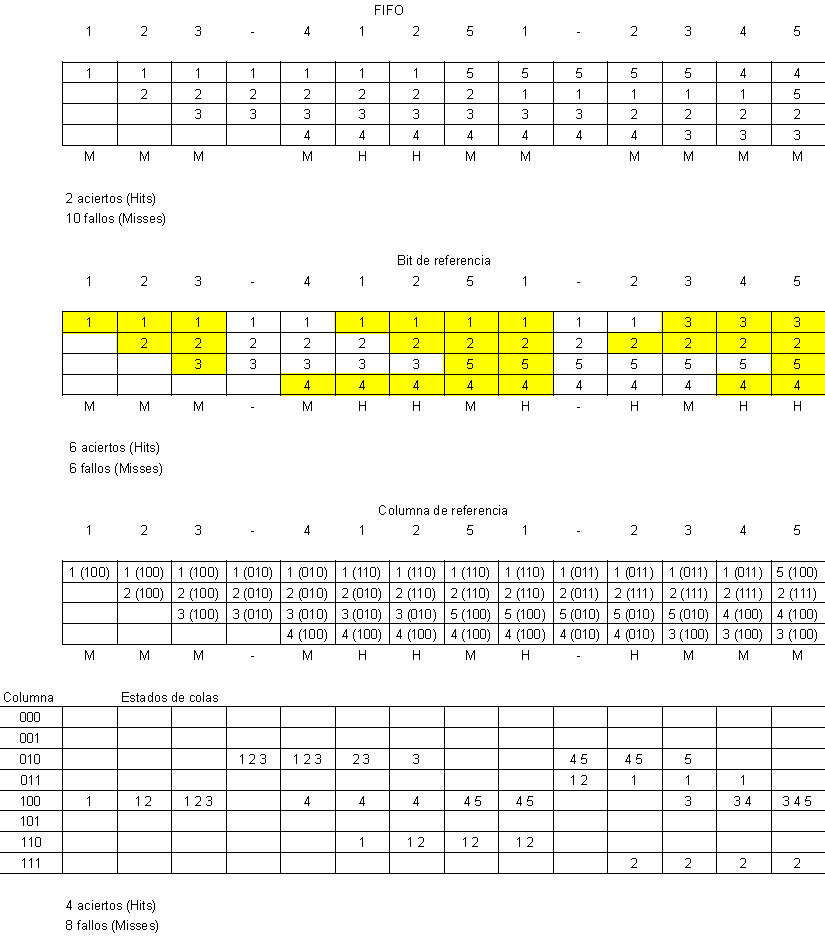
\includegraphics[width=0.85\linewidth]{Paginación.pdf}
  \end{center}
\end{figure}

\end{document}
